\documentclass[12pt]{standalone}
\usepackage{tikz}
\usetikzlibrary{patterns} % calc, arrows.meta, decorations.pathreplacing}

\begin{document}

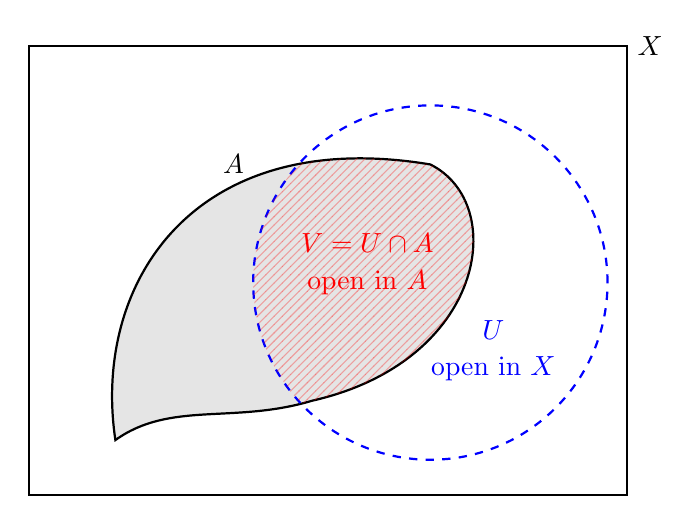
\begin{tikzpicture}%[baseline={(0,0)}]
			% Define the space X as a large rectangle
			\draw[thick] (-3.6, -2.7) rectangle (4, 3) node[anchor=west] {$X$};
			
			% Define the subset A as an irregular shape inside X
			\filldraw[fill=gray!20, draw=black, thick] 
			(-2.5, -2) .. controls (-2.8, 0) and (-1.5, 2) .. (1.5, 1.5)
			.. controls (2.5, 1) and (2.2, -1) .. (0, -1.5)
			.. controls (-1, -1.8) and (-1.8, -1.5) .. cycle;
			\node at (-1, 1.5) {$A$};
			
			% Draw the open set U as a circle inside X
			\draw[thick, blue, dashed] (1.5, 0) circle (2.25); 
			\node[blue] at (2.3,-0.6) {$U$};
			\node[blue] at (2.3,-1.1) {$\mathrm{open\ in\ }X$};
			
			% Draw the intersection V = U ∩ A with a distinct color
			%\fill[red, opacity=0.4] 
			%  (0.25, -0.75) .. controls (0.5, 0) and (1.5, 1.2) .. (1, 0.5)
			%  .. controls (0, -1) and (-0.5, -0.75) .. cycle;
			
			% Add label for V
			\node[red] at (0.7, 0.5) {$V = U \cap A$};
			\node[red] at (0.7, 0.0) {$\mathrm{open\ in\ }A$};
			
			
			% Shade the intersection of U and A
			\clip (1.5, 0) circle (2.25);
			\fill[pattern=north east lines, pattern color=red, opacity=0.3] 
			(-2.5, -2) .. controls (-2.8, 0) and (-1.5, 2) .. (1.5, 1.5)
			.. controls (2.5, 1) and (2.2, -1) .. (0, -1.5)
			.. controls (-1, -1.8) and (-1.8, -1.5) .. cycle;
		\end{tikzpicture}
		%lwarp%\end{lateximage}
			%%%%%%%%%%%%%%%%%%%

\end{document}
